%%%%%%
%
% $Author: Yogesh$
% $Date: 29.04.2024 $
% $Path: BA24-02-Time-Series\report\Contents\en$
% $Version: 1.0 $
% $Reviewed by: Rakesh $
%
% !TeX encoding = utf8
% !TeX root = Rename
% !TeX TXS-program:bibliography = txs:///bibtex
%
%%%%%%

\chapter{Data Version Control}
\section{Introduction}
Data versioning, according to the definition in Stanford libraries, means that
when you make changes to data, a new version and new copies of data are generated,
allowing you to easily rollback and retrieve specific versions of data. A version
is created when there is a change that makes it different from an earlier form.
We can consider it a new version when there is a change in the content or
structure of the source \cite{Zhao:2020}.

In our project, we will apply data versioning techniques to manage the air pollution
data from various sources. This will enable us to track changes and updates in
the datasets over time, ensuring that our analyses are based on consistent and reproducible
data.

\section{Importance of Data Versioning}
Having defined data versioning, it is crucial to understand its importance in
the context of our project. Data versioning is essential for ensuring the accuracy,
reliability, and reproducibility of our research on air pollution. By using
standardized versioning rules, we can track how our datasets evolve and choose specific
versions to work with \cite{Zhao:2020}. Here are some key reasons why dataset
versioning is important in our project:

\begin{enumerate}[label=\textbf{\arabic{*}.}]
	\item \textbf{Reproducibility}: In scientific research and data-driven projects
	like ours, being able to reproduce results is critical. Proper dataset versioning
	allows us to access the exact data used to generate a particular result,
	making it easier to reproduce those results in the future \cite{DVC:2023}.
	
	\item \textbf{Auditability}: When dealing with sensitive or regulated data,
	such as air pollution measurements, it’s important to demonstrate that the data
	hasn’t been tampered with. Dataset versioning helps us track changes over
	time and maintain a clear audit trail \cite{DVC:2023}.
	
	\item \textbf{Historical record}: Data is often an organization’s most important
	asset, and maintaining a reliable historical record is crucial. Dataset versioning
	allows us to track the evolution of our air pollution data, making it easier
	to understand how it has changed and why. This is particularly relevant for adhering
	to regulations like the EU AI Act, which includes specific requirements for
	record keeping \cite{DVC:2023}.
\end{enumerate}

In conclusion, implementing data versioning in our project ensures that our
research on air pollution is reproducible, auditable, and maintains a
comprehensive historical record of our data. This practice not only supports the
integrity of our findings but also facilitates compliance with relevant regulations
and standards.

\section{How to Choose a Data Versioning Tool}

To choose a suitable data versioning tool for your workflow, you should consider
the following factors:

\begin{enumerate}
	\item \textbf{Support for project data modality}: How does it support video/audio?
	Does it provide some preview for tabular data?	
	\item \textbf{Ease of use}: How easy is it to use in project workflow? How
	much overhead does it add to application execution?
	\item \textbf{Diff and compare}: Can we compare datasets? Can we see the diff
	for your image directory?
	\item \textbf{Integration with project stack}: Can we easily connect to your infrastructure,
	platform, or model training workflow?
	\item \textbf{Team adoption}: If your team does not adopt it, it doesn’t
	matter how good the tool is. So keep your teammates' skill sets and
	preferences in mind \cite{DVCTools:2023}.
\end{enumerate}
\section{Tools}
\begin{figure}[H]
	\centering
	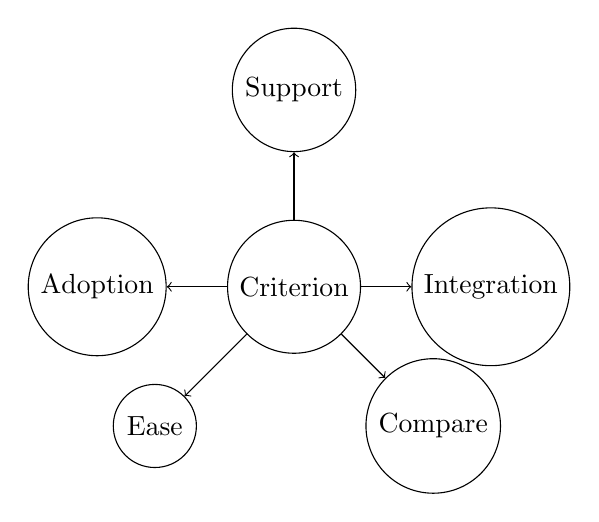
\begin{tikzpicture}[node distance=2.5cm, auto]
		% Define nodes
		\node[draw, circle, align=center] (center) {Criterion}; \node[draw, circle, above
		of=center, align=center] (support) {Support}; \node[draw, circle, below left
		of=center, align=center] (ease) {Ease}; \node[draw, circle, below right of=center,
		align=center] (diff) {Compare}; \node[draw, circle, right of=center, align=center]
		(integration) {Integration}; \node[draw, circle, left of=center, align=center]
		(team) {Adoption};
		
		% Draw edges
		\draw[->] (center) -- (support); \draw[->] (center) -- (ease); \draw[->] (center)
		-- (diff); \draw[->] (center) -- (integration); \draw[->] (center) -- (team);
	\end{tikzpicture}
	\caption{Factors to Consider When Choosing a Data Versioning Tool}
	\label{fig:data_versioning_tool_criteria}
\end{figure}

Let's discuss the tools which we can use for data versioning activities for air
pollution forecasting for Indian dataset
\subsection{Neptune}

Neptune is an ML metadata store built for research and production teams that run
many experiments. It allows logging and displaying various ML metadata, including
hyperparameters, metrics, videos, interactive visualizations, and data versions.Please
refer below sample dashboard fig. \ref{Neptune}.

\begin{figure}[H]
	\centering
	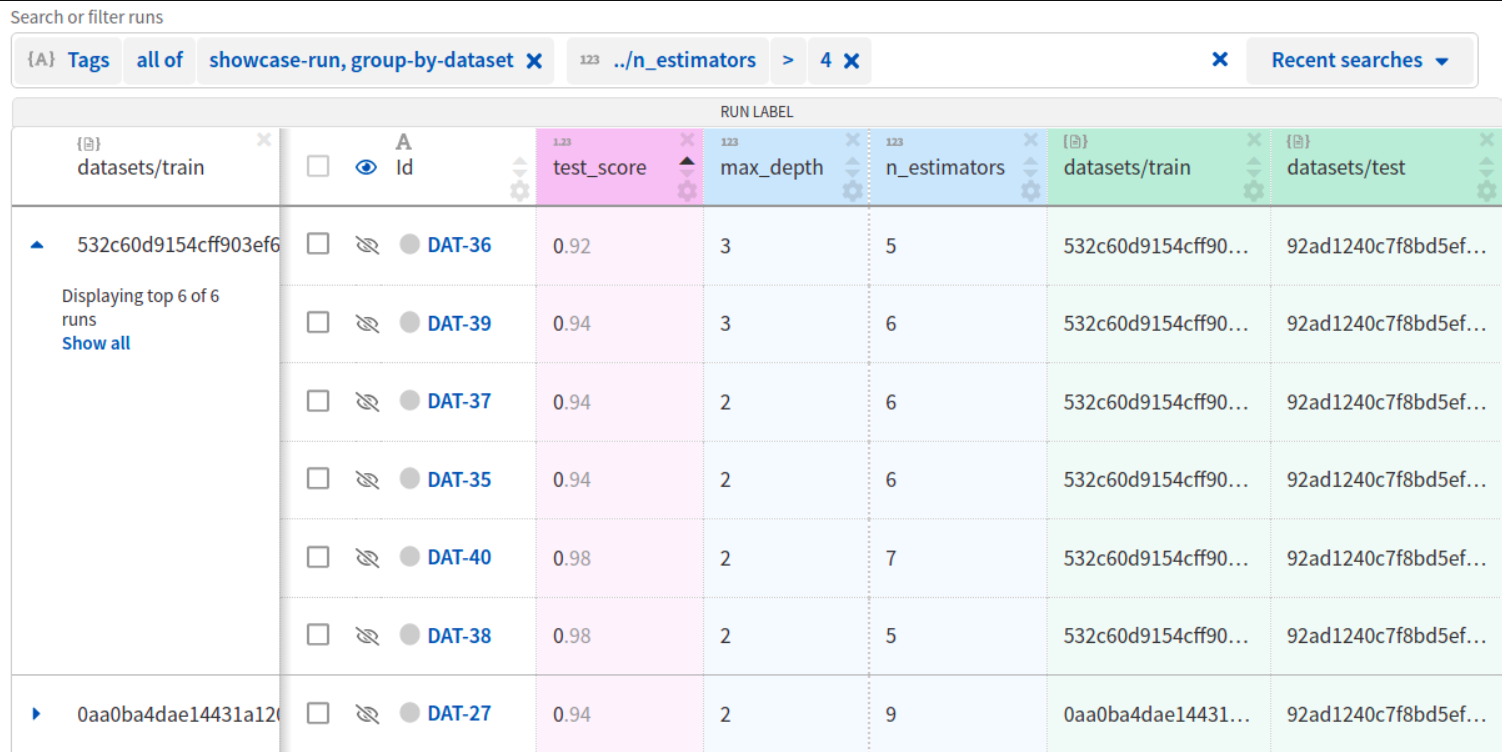
\includegraphics[width=0.8\textwidth]{Images/NeptuneDashboard}
	\caption{Example dashboard in Neptunee}
	\label{Neptune}
\end{figure}

Neptune artifacts let you version datasets, models, and other files from your local
filesystem or any S3-compatible storage with a single line of code. Specifically,
it saves:

\begin{itemize}
	\item Version (hash) for the file or folder
	
	\item Location of the file or folder
	
	\item Folder structure (recursively)
	
	\item Size of the file or folder
\end{itemize}

Once logged, you can use the Neptune UI to group runs on dataset versions or see
how the artifacts changed between runs. Neptune offers a lightweight solution
for data versioning, experiment tracking, and model registry, using a flexible metadata
structure for organizing training and production metadata \cite{DVCTools:2023}.

\textbf{For more information:}
\begin{itemize}
	\item \href{https://neptune.ai/case-studies}{Case studies}
	
	\item \href{https://neptune.ai/project-examples}{Example public projects}
	
	\item \href{https://colab.research.google.com/github/neptune-ai/examples}{Colab
		examples}
\end{itemize}

\subsection{Pachyderm}

Pachyderm is a complete version-controlled data science platform that manages
the end-to-end machine learning lifecycle. It comes in three versions: Community
Edition (open-source), Enterprise Edition (complete platform), and Hub Edition (hosted
version, beta).Please refer below sample dashboard fig. \ref{PACHDASH}.

\begin{figure}[H]
	\centering
	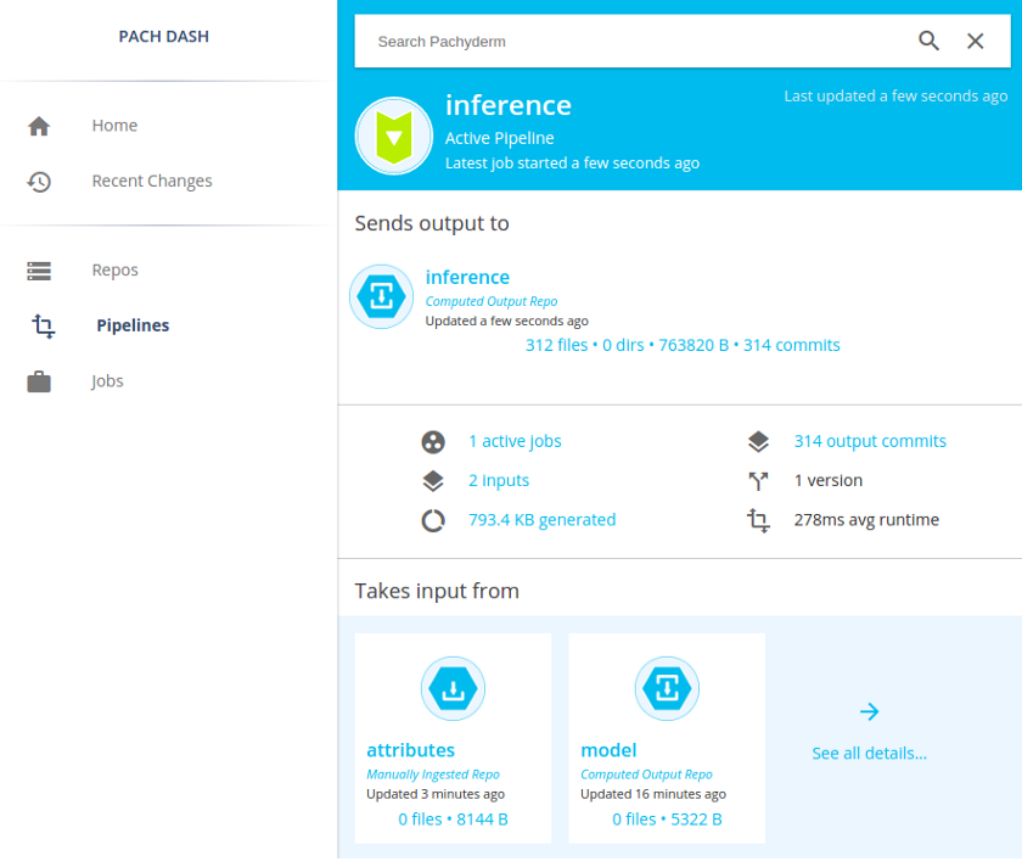
\includegraphics[width=0.8\textwidth]{Images/PachDash}
	\caption{Example dashboard in Pachyderm}
	\label{PACHDASH}
\end{figure}

With Pachyderm, you can:

\begin{itemize}
	\item Continuously update data in the master branch while experimenting with specific
	data commits in separate branches.
	
	\item Support any type, size, and number of files.
	
	\item Ensure centralized and transactional commits.
	
	\item Utilize provenance to maintain a complete audit trail, enabling
	reproducible results \cite{DVCTools:2023}.
\end{itemize}

\textbf{For more information:}
\begin{itemize}
	\item \href{https://www.pachyderm.com}{Pachyderm Official Website}
	
	\item \href{https://www.pachyderm.com/docs}{Pachyderm Documentation}
\end{itemize}

\subsection{DVC}

\begin{figure}[H]
	\centering
	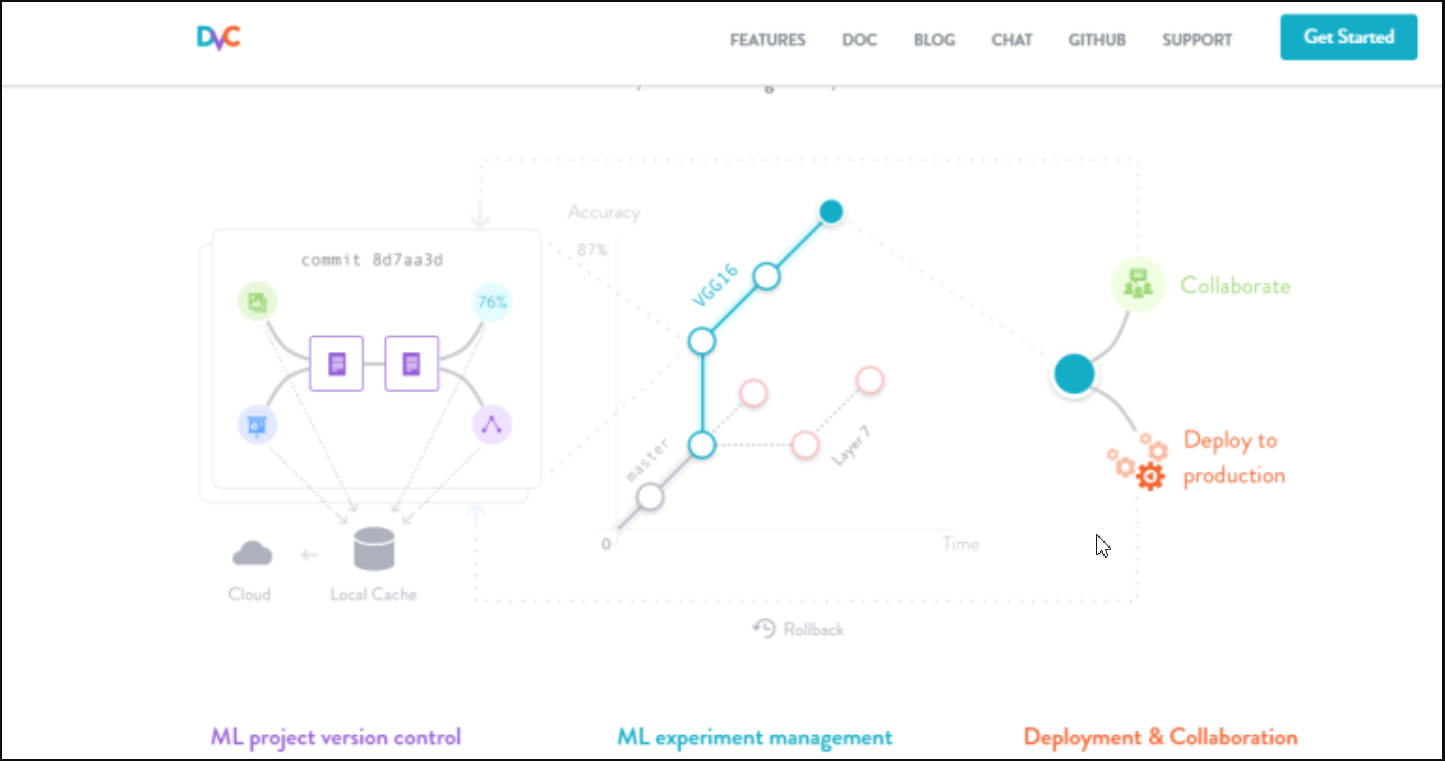
\includegraphics[width=0.8\textwidth]{Images/DVC}
	\caption{DVC Overview}
	\label{DVC}
\end{figure}
DVC is an open-source version control system for machine learning projects. It allows
you to define your pipeline regardless of the language used, offering
reproducibility by leveraging code data and pipeline versioning
\cite{DVCTools:2023}.

DVC features include:

\begin{itemize}
	\item Storage agnostic with support for various types of storage.
	
	\item Full code and data provenance.
	
	\item Consistent reproducibility of experiments.
	
	\item Tracking metrics and failed attempts.
	
	\item Integration with any Git repository.
\end{itemize}

\textbf{For more information:}
\begin{itemize}
	\item \href{https://dvc.org}{DVC Official Website}
	
	\item \href{https://dvc.org/doc}{DVC Documentation}
\end{itemize}

\subsection{Git Large File Storage (LFS)}

\begin{figure}[H]
	\centering
	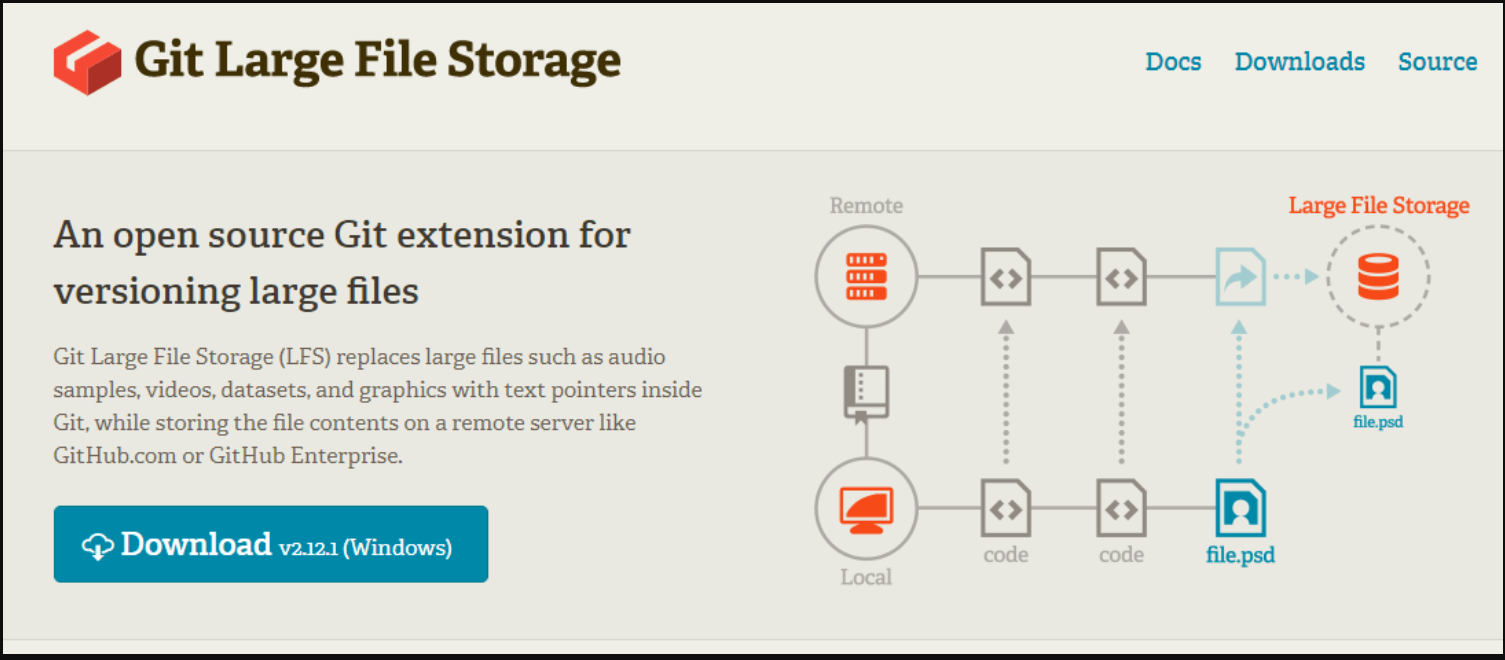
\includegraphics[width=0.8\textwidth]{Images/Git_LFS}
	\caption{Git LFS Overview}
	\label{GitLFS}
\end{figure}

Git LFS is an open-source project that integrates with Git to handle large files
more efficiently. It replaces large files like audio samples, videos, datasets, and
graphics with text pointers inside Git repositories, while storing the actual
file contents on a remote server such as GitHub.com or GitHub Enterprise.

Key features of Git LFS include:

\begin{itemize}
	\item Versioning of large files within Git repositories.
	
	\item External storage for large files, improving repository performance.
	
	\item Faster clone and fetch operations for repositories with large files.
	
	\item Maintains existing workflow and access controls for large files alongside
	other repository content when using remote hosts like GitHub \cite{DVCTools:2023}.
\end{itemize}

\textbf{For more information:}
\begin{itemize}
	\item \href{https://git-lfs.github.com/}{Git LFS Official Website}
	
	\item \href{https://github.com/git-lfs/git-lfs/wiki/Tutorial}{Git LFS
		Documentation}
\end{itemize}

\subsection{Delta Lake}

\begin{figure}[H]
	\centering
	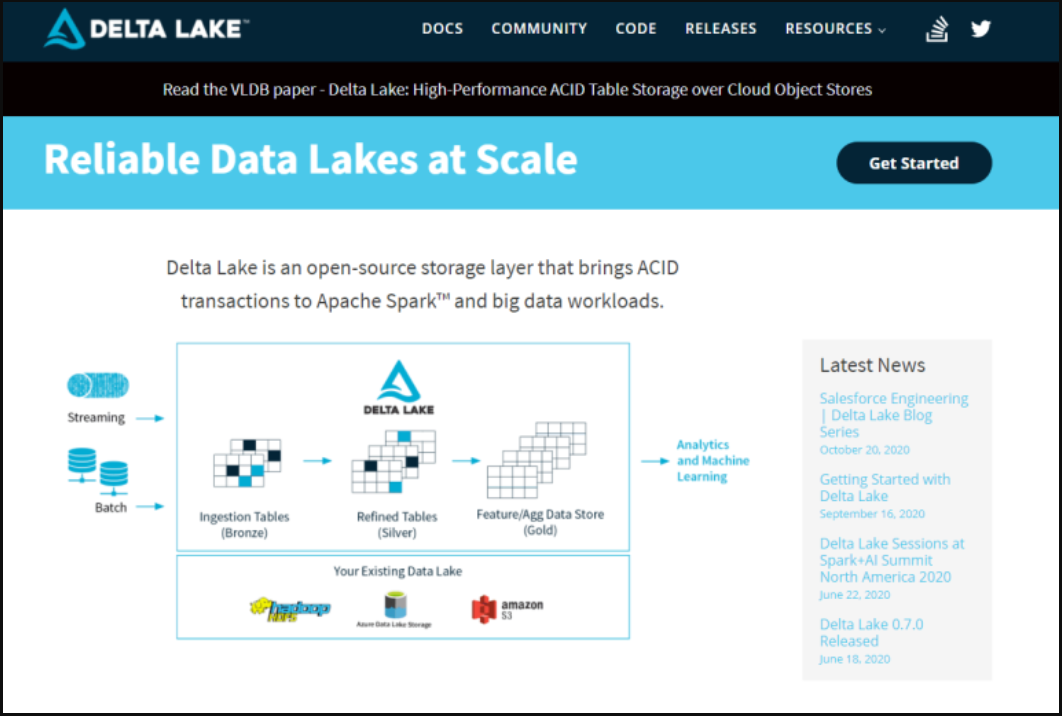
\includegraphics[width=0.8\textwidth]{Images/DeltaLake}
	\caption{Delta Lake Overview}
	\label{DeltaLake}
\end{figure}

Delta Lake is an open-source storage layer designed to bring reliability to data
lakes. It operates on top of existing data lakes and seamlessly integrates with
Apache Spark APIs, offering several key features:

\begin{itemize}
	\item ACID Transactions: Provides Atomicity, Consistency, Isolation, and Durability
	guarantees for data operations.
	
	\item Scalable Metadata Handling: Utilizes Spark's distributed processing
	capabilities to manage metadata efficiently, even for large-scale tables with
	billions of files.
	
	\item Streaming and Batch Unification: Enables a Delta Lake table to function
	as both a batch table and a streaming source/sink, supporting seamless data ingest,
	historic backfill, and interactive queries.
	
	\item Schema Enforcement: Automatically handles schema evolution to maintain
	data quality by preventing insertion of erroneous records during data
	ingestion.
	
	\item Serializable Isolation Levels: Ensures that data read operations are not
	affected by concurrent write operations, maintaining consistency.
	
	\item Data Versioning: Enables rollback capabilities, full historical audit trails,
	and reproducible machine learning experiments by storing data versions.
	
	\item Supports Merge, Update, and Delete Operations: Facilitates complex data
	manipulation tasks such as change-data-capture, slowly-changing-dimension operations,
	and streaming upsert \cite{DVCTools:2023}.
\end{itemize}

\textbf{For more information:}
\begin{itemize}
	\item \href{https://delta.io/}{Delta Lake Official Website}
	
	\item \href{https://docs.delta.io/latest/index.html}{Delta Lake Documentation}
\end{itemize}

\section{Decision}

For our air quality forecasting project in India, we have decided to adopt Git
Large File Storage (LFS) alongside our existing GitHub repository. Git LFS enables
efficient handling of large datasets within Git, integrating seamlessly with
GitHub for versioning and collaboration. This decision ensures our project remains
organized and scalable, leveraging existing tools while managing large files
effectively.